%!TEX root = ../tudkom_students__201804_v1.4.tex
\chapter{Hintergrund}
\label{ch:background}
%This chapter should give a comprehensive overview on the background necessary to understand the thesis.
% 5 pages

\section{Sensor}
Um Gelenkstellungen anzugeben wird eine Position und Rotation gebraucht.
Diese wird von einem Beschleunigungssensor und einem Gyrosensor erfasst und besteht aus je 3 Achsen.
Die Sensoren sind getrennt erhältlich oder zusammen in einer Inertialen Messeinheit (IMU).
Im Folgenden wird ein Einblick in die Funktionsweise der beiden Sensorentypen gegeben.

\subsection{Beschleunigungssensor}
Beschleunigungssensoren können die Beschleunigung messen, die auf den Sensor einwirkt.
Im Bereich der kleinen Bauteile werden zwei Techniken dafür eingesetzt.\\
Beim kapazitiven Sensor, der in Abbildung \ref{fig:pic_accel_kapa} illustriert ist, wird eine Masse senkrecht-federnd parallel zu einer Platte befestigt, mit der sie einen Kondensator bildet.
Bei einer Beschleunigung bewegt sich die Masse zur Platte hin oder davon weg und die Kapazität des Kondensators ändert sich.
Durch diese Änderung lässt sich dann der Wert für die Beschleunigung berechnen.\footnote{\url{https://www.elektronik-kompendium.de/sites/bau/1503041.htm}, aufgerufen am 30.06.2019}
\begin{figure}[h]
	\centering
	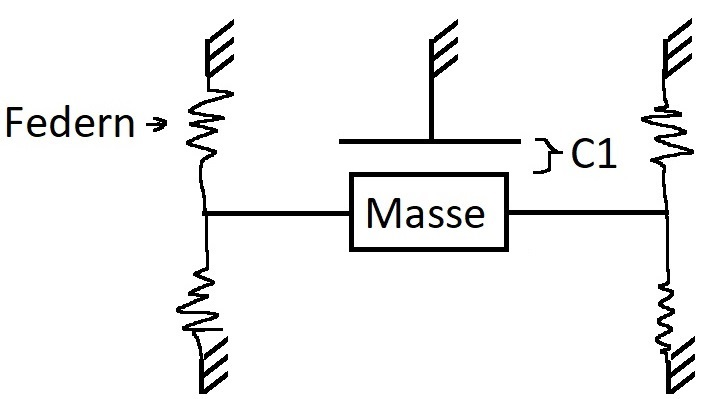
\includegraphics[width=0.33\linewidth]{res/kinAccel.jpg}
	\caption{Kapazitiver Beschleunigungssensor. Basierend auf \url{https://www.sensoren.info/mikromechBeschl.png}, aufgerufen am 30.06.2019}
	\label{fig:pic_accel_kapa}
\end{figure}\\
Beim piezoresistiven Sensor, der in Abbildung \ref{fig:pic_accel_pie} dargestellt ist, wird ein Stoff mit piezoresistivem Effekt genutzt, der bei Dehnung seinen Widerstand ändert.
Eine Masse wird an diesen piezoresistiven Stoff befestigt und durch die Beschleunigung wird der Stoff gedehnt, wodurch durch die Änderung des Widerstands die Beschleunigung berechnet werden kann.\footnote{\url{https://www.elektronik-kompendium.de/sites/bau/1404151.htm}, aufgerufen am 30.06.2019}
\begin{figure}[h]
	\centering
	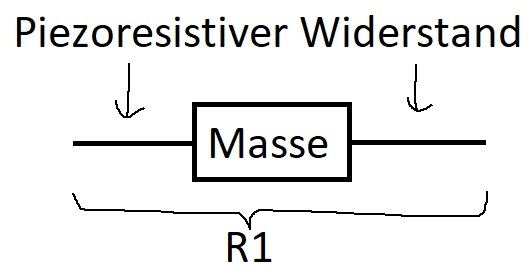
\includegraphics[width=0.25\linewidth]{res/prAccel.jpg}
	\caption{Piezoresistiver Beschleunigungssensor. Basierend auf \url{https://www.sensoren.info/mikromechBeschl.png}, aufgerufen am 30.06.2019}
	\label{fig:pic_accel_pie}
\end{figure}\\

\subsection{Gyrosensor}
Mit einem Gyrosensor, zu sehen in Abbildung \ref{fig:pic_gyro}, wird die Drehung gemessen.
Eine Masse wird dabei senkrecht-federnd parallel zu einer Platte befestigt, sodass wieder ein Kondensator entsteht und parallel zu Dieser von außen zum Schwingen gebracht.
Dieses Konstrukt gibt es ein zweites Mal in die andere Richtung schwingend.
Bei einer Drehung bewegen sich die Masse durch den Coriolis Effekt.
Durch die Subtraktion der beiden Kapazitäten kann man dann die Drehgeschwindigkeit berechnen.
Da die Schwingung gegensätzlich ist, bewegen sich die Massen durch den Coriolis Effekt bei einer Drehung in entgegengesetzte Richtungen und die Differenz der Kapazitäten ändert sich.
Bei einer geraden Beschleunigung bewegen sich beide Massen in die selbe Richtung und die Differenz der Kapazitäten ändert sich nicht. \cite{gyrosensor}
\begin{figure}[h]
	\centering
	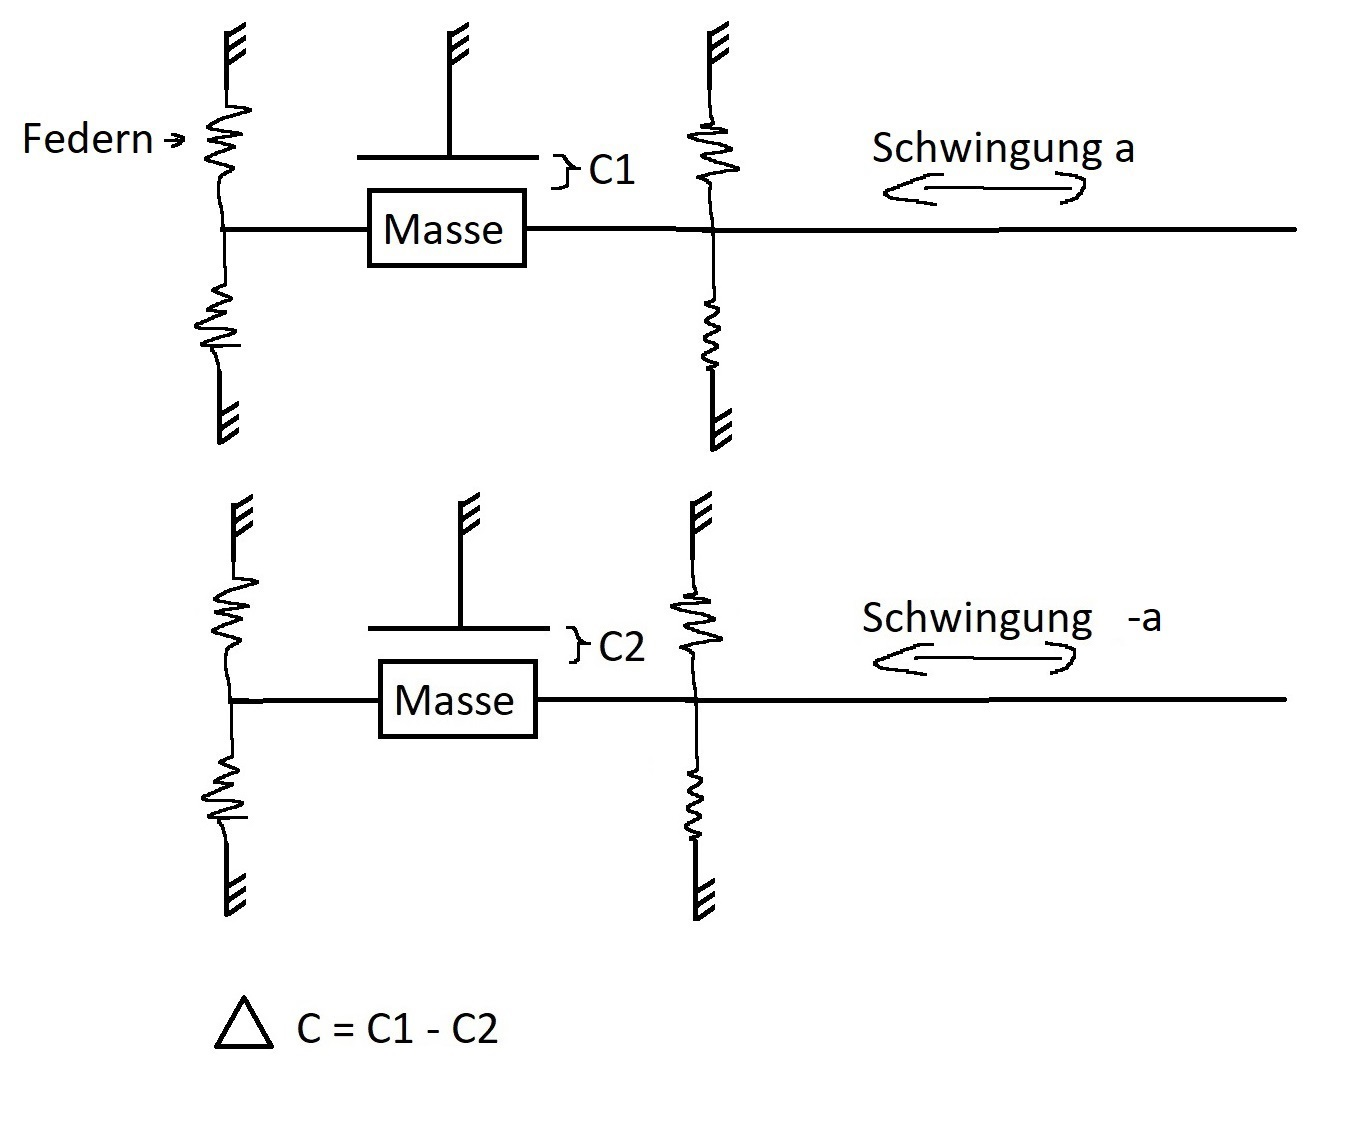
\includegraphics[width=0.65\linewidth]{res/gyro.jpg}
	\caption{Gyrosensor}
	\label{fig:pic_gyro}
\end{figure}\\
Da konstant eine Schwingung auf der Masse gehalten werden muss, damit der Coriolis Effekt auftritt, benötigt der Gyrosensor meist mehr Strom als der Beschleunigungssensor, was später von den Komponenten bestätigt wird.

\section{Datenübertragung zwischen Wearable und Endgerät}
Um das am Besten geeignete Protokoll zu finden, um die Sensordaten der IMU auf die Endgeräte zu übertragen, wurden verschiedene Protokolle verglichen und nach dem Ausschlussverfahren ausgewählt.

\subsection{Vergleich verschiedener Protokolle}
Eine drahtgebundene Datenübertragung ist schnell und sehr energiesparend und über mit z.B. USB ist auch ein weit verbreiteter Anschluss spezifiziert.
Die Mobilität ist dabei aber sehr stark eingeschränkt, da Kabel insbesondere beim Sport sehr stören.\\
Während einige drahtlose Kommunikationsprotokolle wie NFC wegen der geringen Reichweite nicht geeignet sind, sind Mobilfunkprotokolle wie LTE wegen zu hoher Reichweite ineffizient \cite{comparison_wifi_lte}.
Die bekannten Protokolle WIFI und Bluetooth arbeiten unter anderem auf der 2.4-GHz Antenne, weswegen Peer-to-Peer(P2P) Protokolle auf dieser Frequenz in Tabelle \ref{tab:p2p_protocols} vergleichen wurden.
\begin{minipage}{\linewidth}
        \renewcommand\footnoterule{}
        \renewcommand{\thefootnote}{\alph{footnote}}
	\captionof{table}{P2P-Protokolle auf der 2.4-GHz Frequenz}
	\label{tab:p2p_protocols}
	\begin{tabularx}{\linewidth}{>{\hsize=.3\hsize}X|>{\hsize=.5\hsize}X|X}
		Protokoll & Typische Anwendung & Kommentar\\
		\hline
		Wi-Fi Hotspot & Teilen der Internetverbindung in einem lokalem Netzwerk & Am Smartphone kann ein Hotspot erstellt werden, die Wearables könnten diesen suchen und sich verbinden, woraufhin z.B. über eine REST-API kommuniziert werden kann. Es kann auch die 5-GHz Frequenz genutzt werden.\\
		Wi-Fi Direct & P2P-Kommunikation & Wie Wi-Fi Hotspot aber die Wearables bekommen keinen Internetzugriff vom Smartphone.\\
		Bluetooth (BT) & Datenübertragung, Audiostreaming & Nicht für niedrigen Energieverbrauch ausgelegt.\\
		BT Low Energy (BLE) & P2P-Kommunikation mit geringem Energieverbrauch, z.B. Smartwatches & Während die maximale Geräteanzahl nicht vom Protokoll spezifiziert ist, ist diese in Android auf 7 Geräte beschränkt\footnotemark[1]. Weiterhin ist die Anzahl zum Beispiel durch die Auslastung der Geräte und des Funkkanals begrenzt.\\
		BT Mesh & Mesh-Kommunikation mit geringem Energieverbrauch & Nachrichten werden hierbei über das gesamte Netzwerk geflutet, wodurch die Reichweite des Netzwerkes erhöht wird und die Auslastung auf das Netzwerk verteilt wird aber der Energieverbrauch aller Knoten steigt. BLE Geräte können mit Mesh-Netzwerken kompatibel gemacht werden, indem sie sich zu einem Knoten des Netzwerks verbinden.\\
		Thread, ZigBee & Smarthome & Nicht ohne weitere Hardware unter Android\\
		Ant, Ant+ & Sen\-sor\-da\-ten\-über\-tra\-gung mit geringem Energieverbrauch & Nicht von allen Smartphones ohne zusätzliche Hardware unterstützt\\
	\end{tabularx}
	\footnotetext[1]{Beschränkung durch GATT\_MAX\_PHY\_CHANNEL: \url{https://android.googlesource.com/platform/external/bluetooth/bluedroid/+/master/include/bt\_target.h\#1428}}
\end{minipage}\\\\
Da Bluetooth nicht für einen geringen Energieverbrauch ausgelegt ist, werden die Alternativen BLE und BT Mesh bevorzugt.
Die Smarthome Protokolle funktionieren ohne zusätzlicher Hardware nicht am Smartphone.
Ant und Ant+ sind zwar für die Sensordatenübertragung bei Smartphones ausgelegt, aber brauchen zusätzlich ein Dongle, wenn diese das Protokoll nicht unterstützen.
Sowohl handelsübliche Laptops als auch das vorliegende Smartphone, ein Pocophone F1, unterstützt die Protokolle nicht.\\
"BLE ist etwa 30\% energieeffizienter als Wi-Fi"\footnote{Übersetzung durch den Verfasser} \cite{comparison_wifi_ble}, weswegen die Wi-Fi Protokolle heraus fallen.
BT Mesh löst zwar das Problem der Geräteanzahlbeschränkung unter Android, allerdings auf Kosten des Energieverbrauchs.
Die erweiterte Reichweite wird bei einem Wearable in der Regel nicht benötigt.\\
Dem Ausschlussverfahren nach soll die Datenübertragung zwischen Wearable und Endgerät mit BLE stattfinden, da dieses Protokoll von fast jedem Smartphone und Laptop unterstützt wird und den Anforderungen am Besten entspricht.

\subsection{Bluetooth Low Energy}
BLE ist eine Abwandlung von Bluetooth, die für geringen Energieverbrauch optimiert ist.
Geräte können dabei die Rolle vom Central oder Peripheral einnehmen, die einem Master-Slave Protokoll gleichkommen.
Um eine Datenverbindung zu starten, kündigt sich die Peripheral auf den drei Advertising Frequenzen an und die Central hört diese ab.
Die Parameter dafür, zum Beispiel die bis zu 31 Byte große Payload, werden im Generic Access Profile (GAP) eingestellt.
Die Central kann auf die Ankündigung der Peripheral antworten und sich mit Diesem verbinden.\footnote{\url{https://cdn-learn.adafruit.com/downloads/pdf/introduction-to-bluetooth-low-energy.pdf?timestamp=1562415841}, aufgerufen am 06.07.2019}\\
Nach dem Verbindungsaufbau gibt die Central eine Geschwindigkeit vor.
Die Geschwindigkeit besteht aus einem Connection Interval, einer Slave Latency und einem Supervision Timeout.
Das Connection Interval beschreibt in welchen Zeitabständen die Datenbursts passieren.
Sie liegt zwischen 7.5 ms und 4 s.
Die Slave Latency bestimmt, wie oft das Peripheral die Datenbursts pausieren kann um Energie zu sparen, falls keine Daten gesendet werden müssen.
Die Supervision Timeout besagt, nach welcher Zeit eine Verbindung als abgebrochen gilt, wenn eine Seite nicht mehr antwortet.
Später kann einerseits die Peripheral neue Geschwindigkeiten vorschlagen, die von der Central angenommen oder abgelehnt werden oder andererseits die Central neue Geschwindigkeiten von sich aus bestimmen.\footnote{\url{http://dev.ti.com/tirex/content/simplelink\_cc2640r2\_sdk\_1\_40\_00\_45/docs/blestack/ble\_user\_guide/html/ble-stack-3.x/gap.html\#}, aufgerufen am 06.07.2019}\\
Bei einer Verbindung stellt die Peripheral Services zur Verfügung, die aus Characteristics bestehen.
Jede Service und Characteristic hat dabei eine eindeutige UUID.
Diese ist 16 Bit groß, wenn sie aus den vordefinierten Profilen besteht oder 128 Bit für eigene Definitionen.
Eine Characteristic repräsentiert einen Wert und kann im Lese- und Schreibzugriff eingeschränkt werden.
Die Central kann das notificate- oder indicate-Bit setzen, wodurch die Peripheral Änderungen des Wertes mitteilt, wobei beim Indicate der Empfang der Updates von der Central bestätigt werden muss.\footnote{\url{https://devzone.nordicsemi.com/nordic/short-range-guides/b/bluetooth-low-energy/posts/ble-characteristics-a-beginners-tutorial}, aufgerufen am 06.07.2019}\\

\section{Chipkommunikation}
Eine IMU enthält in der Regel keine programmierbare Chiparchitektur sondern wird mit einer Microprocessor Unit (MPU) betrieben.
Diese beinhaltet unter anderem eine Recheneinheit und einen Programmspeicher.
Zur Kommunikation zwischen IMU und MPU kann man wiederum zwischen einigen Protokollen wählen.
Die verwendeten IMUs unterstützen die weit verbreiteten Protokolle Inter-Integrated Circuit (I2C) und Serial Peripheral Interface (SPI), die auch Beide auf der gewählten MPU laufen.
Die Chipkommunikation läuft in der Regel mit einer langsameren Frequenz als die Recheneinheit.
Einerseits kann die Protokollfrequenz von der Software emuliert werden, indem Takte der Recheneinheit übersprungen werden, wodurch die Recheneinheit nicht in den Schlafmodus gehen kann.
Andererseits kann die Recheneinheit einen weiteren Chip nutzen, der mit einem Buffer die Protokolle effizient abarbeiten kann.
\\
In \cite{comparison_i2c_spi} wurde ermittelt, dass I2C einen doppelt so hohen Energieverbrauch wie SPI hat.
Da die Protokolle nur vorschreiben wie Daten gesendet werden, aber die Informationen implementierungsabhängig ineffizient verpackt werden können, wurden beide Protokolle mit dem Wearable getestet.\\

\subsection{SPI}

\subsection{I2C}

\section{Energieversorgung}
nickel und lithium. akku und batterie.\\
was ist das alles. kleiner vergleich. was wählen wir...

\section{Verfügbare fertige Einheiten}
z.b. TI CC2650STK\\
blabla datenblatt blabla größe blabla überladen blabla überteuert blabla standbystromverbrauch blabla "no longer available for shipment to Europe" ggwp\\
\\
oder ACNSENSA\\
blabla datenblatt blabla standbystromverbrauch blabla eingeschränkte verfügbarkeit (datenblatt-links alle down, wtf)
